% Options for packages loaded elsewhere
\PassOptionsToPackage{unicode}{hyperref}
\PassOptionsToPackage{hyphens}{url}
%
\documentclass[
  spanish,
]{book}
\usepackage{amsmath,amssymb}
\usepackage{lmodern}
\usepackage{ifxetex,ifluatex}
\ifnum 0\ifxetex 1\fi\ifluatex 1\fi=0 % if pdftex
  \usepackage[T1]{fontenc}
  \usepackage[utf8]{inputenc}
  \usepackage{textcomp} % provide euro and other symbols
\else % if luatex or xetex
  \usepackage{unicode-math}
  \defaultfontfeatures{Scale=MatchLowercase}
  \defaultfontfeatures[\rmfamily]{Ligatures=TeX,Scale=1}
\fi
% Use upquote if available, for straight quotes in verbatim environments
\IfFileExists{upquote.sty}{\usepackage{upquote}}{}
\IfFileExists{microtype.sty}{% use microtype if available
  \usepackage[]{microtype}
  \UseMicrotypeSet[protrusion]{basicmath} % disable protrusion for tt fonts
}{}
\makeatletter
\@ifundefined{KOMAClassName}{% if non-KOMA class
  \IfFileExists{parskip.sty}{%
    \usepackage{parskip}
  }{% else
    \setlength{\parindent}{0pt}
    \setlength{\parskip}{6pt plus 2pt minus 1pt}}
}{% if KOMA class
  \KOMAoptions{parskip=half}}
\makeatother
\usepackage{xcolor}
\IfFileExists{xurl.sty}{\usepackage{xurl}}{} % add URL line breaks if available
\IfFileExists{bookmark.sty}{\usepackage{bookmark}}{\usepackage{hyperref}}
\hypersetup{
  pdftitle={BioVirología: La biología de los virus},
  pdfauthor={Aimer G. Diaz},
  pdflang={es},
  hidelinks,
  pdfcreator={LaTeX via pandoc}}
\urlstyle{same} % disable monospaced font for URLs
\usepackage{longtable,booktabs,array}
\usepackage{calc} % for calculating minipage widths
% Correct order of tables after \paragraph or \subparagraph
\usepackage{etoolbox}
\makeatletter
\patchcmd\longtable{\par}{\if@noskipsec\mbox{}\fi\par}{}{}
\makeatother
% Allow footnotes in longtable head/foot
\IfFileExists{footnotehyper.sty}{\usepackage{footnotehyper}}{\usepackage{footnote}}
\makesavenoteenv{longtable}
\usepackage{graphicx}
\makeatletter
\def\maxwidth{\ifdim\Gin@nat@width>\linewidth\linewidth\else\Gin@nat@width\fi}
\def\maxheight{\ifdim\Gin@nat@height>\textheight\textheight\else\Gin@nat@height\fi}
\makeatother
% Scale images if necessary, so that they will not overflow the page
% margins by default, and it is still possible to overwrite the defaults
% using explicit options in \includegraphics[width, height, ...]{}
\setkeys{Gin}{width=\maxwidth,height=\maxheight,keepaspectratio}
% Set default figure placement to htbp
\makeatletter
\def\fps@figure{htbp}
\makeatother
\setlength{\emergencystretch}{3em} % prevent overfull lines
\providecommand{\tightlist}{%
  \setlength{\itemsep}{0pt}\setlength{\parskip}{0pt}}
\setcounter{secnumdepth}{5}
\usepackage{booktabs}
\ifxetex
  % Load polyglossia as late as possible: uses bidi with RTL langages (e.g. Hebrew, Arabic)
  \usepackage{polyglossia}
  \setmainlanguage[]{spanish}
\else
  \usepackage[main=spanish]{babel}
% get rid of language-specific shorthands (see #6817):
\let\LanguageShortHands\languageshorthands
\def\languageshorthands#1{}
\fi
\ifluatex
  \usepackage{selnolig}  % disable illegal ligatures
\fi
\usepackage[]{natbib}
\bibliographystyle{apalike}

\title{BioVirología: La biología de los virus}
\author{Aimer G. Diaz}
\date{©2019, All rights reserved.}

\begin{document}
\maketitle

{
\setcounter{tocdepth}{1}
\tableofcontents
}
\hypertarget{bienvenidos-al-bookdown-de-biovirologuxeda}{%
\chapter{Bienvenidos al bookdown de BioVirología}\label{bienvenidos-al-bookdown-de-biovirologuxeda}}

El Blog en Facebook \href{https://www.facebook.com/BioViral/}{Biovirología} se ha mudado a un sitio web más profesional, el formato de libros electrónicos nada tradicional, que hace a los libros electrónicos interactivos: Bookdown. Así con esta transición BioViral se convierte en el primer blog en hacerse libro electrónico interactivo de virología biológica o biovirología y a su vez, en el primer bookdown en hacer divulgación científica en español sobre virología.

El proyecto inició en un nada remoto \href{https://www.facebook.com/permalink.php?story_fbid=107125457678944\&id=107088044349352}{19 de mayo del 2020} con el siguiente post reproducido a continuación:

Inauguro este espacio de divulgación científica en español sobre artículos de investigación en virología desde una perspectiva netamente biológica. En este espacio los virus no solo serán agentes etiológicos o factores causales de enfermedades en humanos; en vez de esto se discutirán como los virus que fungen como nanobiota, son componentes esenciales de nuestra microbiota.
Sobra decirlo, a la pregunta si los virus ¿ viven o no ?. La respuesta es un contundente Si, en palabras del virólogo Frances Patrick Forterre:

``(Los) virus no deben confundirse con sus viriones, sino que se pueden ver como entidades vivientes complejas que transforman la célula infectada en un organismo nuevo, el virus, que produce viriones.''

``Viruses are no more confused with their virions, but can be viewed as complex living entities that transform the infected cell into a novel organism---the virus---producing virions'' \citet{forterre2010defining}

Por la anterior cita, las historias que se contarán serán sobre las fábricas virales (viriones replicantes o una vez germinados en células) y no a las semillas proteicas (viriones) a las que llamaremos virucélulas (virocells). \citet{mukhopadhyay2003structure}

\begin{figure}
\centering
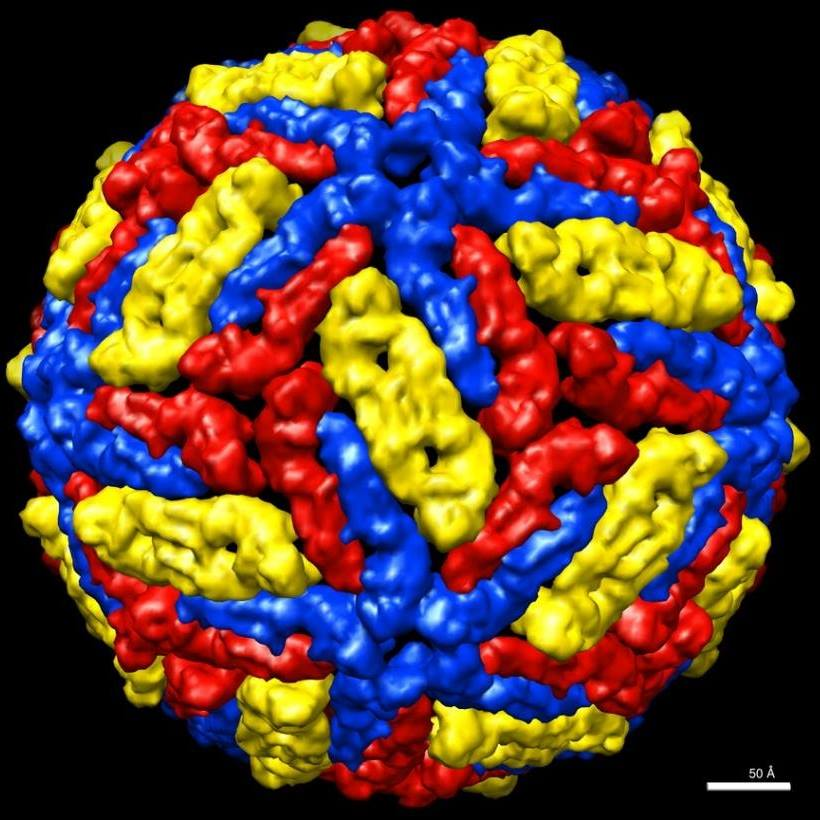
\includegraphics{./165496377_134509338676384_4186488905084681632_n.jpg}
\caption{Partícula viral o virión del virus del Nilo Occidental con los colores del la bandera de Colombia en homenaje al 3 encuentro panamericano de Dengue celebrado en Cartagena Colombia. Autores \citet{mukhopadhyay2003structure}}
\end{figure}

A manera introductoria tanto de las maravillas del formato empleado, los invito a ver el siguiente video con el que puede llevarse una idea inicial del autor del presente bookdown:

\begin{figure}
\centering
\includegraphics[width=0.9\textwidth,height=\textheight]{https://youtu.be/EmEhFhQpqTQ}
\caption{En el color de las plantas, 1 + 1 no es 2}
\end{figure}

\hypertarget{los-virus-son-nano-organismos-y-constituyen-un-imperio-de-la-vida}{%
\chapter{Los virus son nano-organismos y constituyen un imperio de la vida}\label{los-virus-son-nano-organismos-y-constituyen-un-imperio-de-la-vida}}

\hypertarget{quuxe9-son-los-virus-genes-escapados-cuxe9lulas-reducidas-o-las-primeras-cuxe9lulas-que-se-dispersan-con-semillas}{%
\section{¿Qué son los virus? ¿Genes escapados, células reducidas o las primeras células que se dispersan con ``semillas''?}\label{quuxe9-son-los-virus-genes-escapados-cuxe9lulas-reducidas-o-las-primeras-cuxe9lulas-que-se-dispersan-con-semillas}}

\url{https://www.facebook.com/permalink.php?story_fbid=145223737202449\&id=107088044349352}

\hypertarget{los-virus-y-el-color-de-las-plantas}{%
\chapter{Los virus y el color de las plantas}\label{los-virus-y-el-color-de-las-plantas}}

\hypertarget{la-primera-burbuja-especulativa-y-el-virus-del-mosaico-del-tulipan.}{%
\section{La primera burbuja especulativa y el virus del mosaico del tulipan.}\label{la-primera-burbuja-especulativa-y-el-virus-del-mosaico-del-tulipan.}}

\url{https://www.facebook.com/BioViral/posts/166521528808498}

En épocas de pandemia viral se hacen más populares frases negativas en torno a los virus tales como la ya famosa cita del premio nobel de medicina Peter Medawar:

{[}Un virus es{]} ``una mala noticia envuelta en una cubierta de proteína''.

Quizá la popularidad de este tipo de creencias nos impide explorar estos seres vivos tan incomprendidos; de hecho, no resulta extraño que la mayoría aplastante de investigaciones en virología sean del índole médico. Quizá si nos enfocamos primero en entender y no en cómo eliminar, podríamos prevenir de una mejor manera las futuras crisis sanitarias que los virólogos y epidemiólogos YA anticipan.

Para ejemplificar la otra cara de la virología, un aspecto de interés de la virología básica --- y de poca relevancia para la virología médica ---, se encuentra el virus del mosaico del tulipán. Este es uno de los encargados de embellecer aún más el panorama de colores florales de algunas plantas en primavera, esto al incidir en la inhibición de la maquinaria regulatoria mediada por pequeños RNAs, que a su vez inhibe la producción de ciertas enzimas involucradas en la biosíntesis de flavonoides, los pigmentos vegetales que otorgan las coloraciones con tonos amarillas, verdes, púrpuras, azules y rojizas.

En lo que respecta a colores florales, ``menos por menos es más'': durante la infección a la planta huésped, el virus inhibe una de las maquinarias que despliega la planta para su control, los pequeños ARNs de interferencia (small interference RNAs o sRNAi), que a su vez inhibe la expresión de los genes blancos, por complementariedad con el pequeño ARN. Dentro de la lista de genes blancos se encuentran aquellos que promueven la biosíntesis de los pigmentos previamente mencionados. La infección del virus altera esta inhibición, permitiendo expresar en aquellas células infectadas los pigmentos que otorgan la coloración; generando patrones contrastantes entre células infectadas y no infectadas (Figura 3).

Este efecto visual, hizo que el virus del mosaico del tulipán, desatara no una pandemia, pero sí la admiración y la codicia humana que desencadenó la primera crisis económica del viejo mundo: la Tulipomanía del 1637; ejemplificando cómo los virus hacen parte de la biosfera entera, capaz de alterar interacciones ecológicas antiguas o novedosas, y de paso, el sistema económico humano.

\hypertarget{infecciones-virales-a-simple-vista}{%
\section{Infecciones virales a simple vista}\label{infecciones-virales-a-simple-vista}}

\url{https://www.facebook.com/permalink.php?story_fbid=116167563441400\&id=107088044349352}

\hypertarget{el-viroma-humano}{%
\chapter{El viroma humano}\label{el-viroma-humano}}

\hypertarget{el-viroma-del-genoma-humano}{%
\section{El viroma del genoma humano}\label{el-viroma-del-genoma-humano}}

\hypertarget{somos-huxedbridos-entre-virus-y-humanos}{%
\section{¿ Somos híbridos entre virus y humanos ?}\label{somos-huxedbridos-entre-virus-y-humanos}}

\hypertarget{metafuxedsica-y-virologuxeda}{%
\chapter{Metafísica y Virología}\label{metafuxedsica-y-virologuxeda}}

\hypertarget{los-virus-desde-la-ontologuxeda-de-procesos.}{%
\section{Los virus desde la ontología de Procesos.}\label{los-virus-desde-la-ontologuxeda-de-procesos.}}

\hypertarget{muxe1s-alluxe1-de-la-virologuxeda-y-la-ciencia-implicaciones-sociales-de-la-virologuxeda}{%
\chapter{Más allá de la virología y la ciencia: implicaciones sociales de la virología}\label{muxe1s-alluxe1-de-la-virologuxeda-y-la-ciencia-implicaciones-sociales-de-la-virologuxeda}}

\hypertarget{la-extinciuxf3n-del-virus-de-la-viruela-y-el-optimismo-cientificista}{%
\section{La extinción del virus de la viruela y el optimismo cientificista}\label{la-extinciuxf3n-del-virus-de-la-viruela-y-el-optimismo-cientificista}}

\hypertarget{la-pandemia-de-sars-cov-2-el-virus-que-detuvo-un-mundo-hiperglobalizado.}{%
\chapter{La pandemia de SARS-CoV-2: El virus que detuvo un mundo hiperglobalizado.}\label{la-pandemia-de-sars-cov-2-el-virus-que-detuvo-un-mundo-hiperglobalizado.}}

  \bibliography{book.bib,packages.bib,References\_Bibtex.bib}

\end{document}
